\documentclass[10pt,twocolumn,letterpaper]{article}

\usepackage{cvpr}
\usepackage{times}
\usepackage{epsfig}
\usepackage{graphicx}
\usepackage{amsmath}
\usepackage{amssymb}

% Include other packages here, before hyperref.

% If you comment hyperref and then uncomment it, you should delete
% egpaper.aux before re-running latex.  (Or just hit 'q' on the first latex
% run, let it finish, and you should be clear).
\usepackage[breaklinks=true,bookmarks=false]{hyperref}

\cvprfinalcopy % *** Uncomment this line for the final submission

\def\cvprPaperID{****} % *** Enter the CVPR Paper ID here
\def\httilde{\mbox{\tt\raisebox{-.5ex}{\symbol{126}}}}

% Pages are numbered in submission mode, and unnumbered in camera-ready
%\ifcvprfinal\pagestyle{empty}\fi
\begin{document}

%%%%%%%%% TITLE
\title{Luo's part about the computer vision survey}
\author{Ruiqi Luo\\
		16064455\\
		Shanghaitech University\\
		Huanke Rd No.199, Zhangjiang, Pudong district, Shanghai, China\\
		{\tt\small luorq@shanghaitech.edu.cn}
}

\maketitle
%\thispagestyle{empty}

%%%%%%%%% BODY TEXT
\section{Part III: CNN in medical image classification}

%-------------------------------------------------------------------------
\subsection{introduction}

Convolutional neural networks (CNNs) have been used in the field of computer vision for decades. However, their true value had not been discovered until the ImageNet competition in 2012, a success that brought about a revolution through the efficient use of graphics processing units (GPUs), rectified linear units, new dropout regularization, and effective data augmentation. Acknowledged as one of the top 10 breakthroughs of 2013, CNNs have once again become a popular learning machine, now not only within the computer vision community but across various applications ranging from natural language processing to hyperspectral image processing and to medical image analysis. The main power of a CNN lies in its deep architecture, which allows for extracting a set of discriminating features at multiple levels of abstraction\cite{tajbakhsh2016convolutional}. 

However, training a deep CNN with full training is very complicated. First, CNNs require a large
amount of labeled training data. Second, training a deep CNN requires extensive computational and memory resources, without that the training process would be extremely time-consuming.Third, training a deep CNN is often complicated by overfitting. Therefore, deep learning from scratch can be tedious and time-consuming, demanding a great deal of diligence, patience, and expertise.

In this survey, I conducted an extensive set of experiments for 4 medical imaging applications: 1) polyp detection in colonoscopy videos~\cite{ribeiro2016colonic}\cite{zhang2017automatic}, 2) image quality assessment and classification in tissues and cells such as blood vessels videos\cite{mcilroy2017vivo}\cite{li2017cell}\cite{huang2017epithelium}\cite{kieffer2017convolutional}\cite{hadad2017classification}\cite{araujo2017classification}, 3) lung disease such as pulmonary embolism detection and so on in computed tomography (CT) images\cite{shen2015multi}\cite{li2014medical},4) dental disease in X-ray image\cite{prajapaticlassification} and 5) intima-media boundary segmentation in ultrasonographic images\cite{roth2015anatomy}.

\subsection{Polyp detection}

Colorectal cancer (CRC) is one of the leading causes of deathworldwide with about estimated 700 thousand deaths in 2012\cite{zhang2017automatic}. Long-term follow-up studies confirmed that removal of adenomatous polyps reduces CRC mortality. Colonoscopy is the preferred technique for colon cancer screening and prevention. The goal of colonoscopy is to find and remove colonic polyps—precursors to colon cancer. But polyps can appear with substantial variations in color, shape, and size. The challenging appearance of polyps can often lead to misdetection\cite{ribeiro2016colonic}. Polyp miss-rates are estimated to be about 4\% to 12\%; however, a more recent clinical study is suggestive that this misdetection rate may be as high as 25\%. So nowadays, there are many research groups start to use computer aided method such as CNN.

In the article\cite{ribeiro2016colonic}, the author have a small dataset, which only have 100 images(75 abnormal images and 25 healthy images). After finishing the data augmentation which results in 800 images, they resized the 256*256 image to 128*128. In order to test the five architecture they established, he used cross validation method(56 for training and 6 for testing), the result can be seen in Figure 1, the accuracy is just 75\% to 80\%.

\begin{figure}[t]
	\begin{center}
		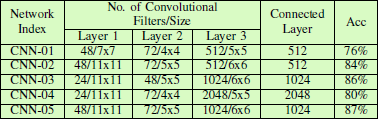
\includegraphics[width=0.8\linewidth]{4}
	\end{center}
	\caption{Accuracy results from different CNN configurations} 
	\label{fig:long}
	\label{fig:onecol}
\end{figure}

In order to improve the accuracy, in the evaluation phase, the author obtained the final decision for a 256*256 pixel image by majority voting of the decisions of all 128*128 pixel subimages(patches). This is a kind of fine-tuning. The redundancy of overlapping subimages can increase the system accuracy likewise to give the assurance of certainty for the overall decision. The result can be seen in figure 2. They also perform a random patch extraction and it can be concluded that there is not much difference between 16384 subimages or
just 32 subimages (accuracy of 90.96\%), saving considerable computation time and achieving good results.

\begin{figure}[t]
	\begin{center}
		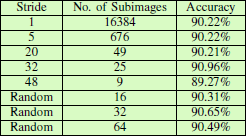
\includegraphics[width=0.8\linewidth]{5}
	\end{center}
	\caption{Accuracy of different strides for overlapping subimages in the evaluation.} 
	\label{fig:long}
	\label{fig:onecol}
\end{figure}

In the second article\cite{zhang2017automatic}, the author use a small datasets(PHW Database), this dataset consisted of 1104, 263 and
563 images without polyps, with hyperplasia polyps and adenomatous polyps, respectively, taken under either WL or NBI endoscopy. For fair comparison, 50 images from each class (nonpolyp, hyperplasia, and adenoma) were randomly selected as testing dataset, while the rest were treated as training dataset.

Because this dataset has an imbalanced number of images for each class, Previous study for polyp detection proposed to use an up/down sampling strategy to tackle such challenge. In this paper, the authors randomly down sampled the majority class to match the sample size of the minority class for both target tasks. The source dataset used ILSVRC and Places205 and trained for 450 000 iterations. They tested two tasks using this database, first is polyp detection and second polyp type classification. In order to do the evaluation, the authors used a feature engineering technique: bag-of-words for comparison. After finishing these tasks, we can see the results in the Figure 3.4.5. In these figures, we can see that transferring low-level CNN features gives better transfer learning performance for both target tasks and when a CNN structure is directly
used for detection and classification. The performance of the proposed method is better in both tasks.

\begin{figure}[t]
	\begin{center}
		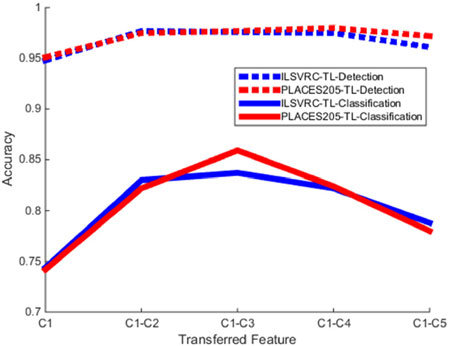
\includegraphics[width=0.8\linewidth]{6}
	\end{center}
	\caption{Average accuracy of the detection and classification tasks by transferring C1–Cn features learned from ILSVRC and Places205 and using SVM as the classifier with a RBF kernel.} 
	\label{fig:long}
	\label{fig:onecol}
\end{figure}

\begin{figure}[t]
	\begin{center}
		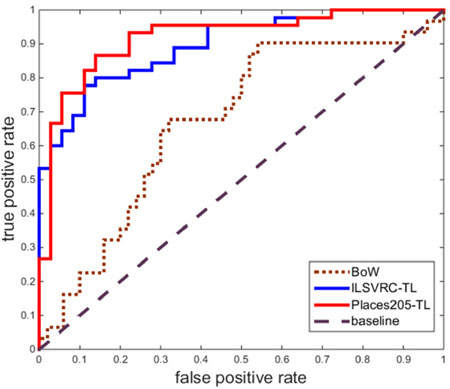
\includegraphics[width=0.8\linewidth]{7}
	\end{center}
	\caption{Typical ROC curve for polyp classification for PWH database.} 
	\label{fig:long}
	\label{fig:onecol}
\end{figure}

\begin{figure}[t]
	\begin{center}
		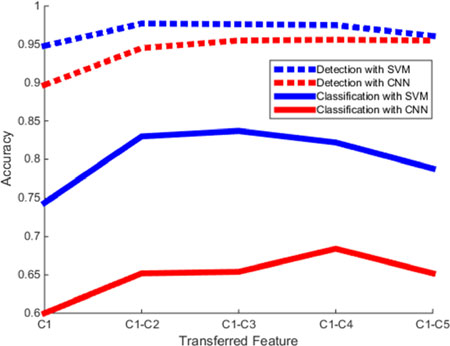
\includegraphics[width=0.8\linewidth]{8}
	\end{center}
	\caption{Average accuracy of the detection and classification tasks by transferring C1–Cn features learned from ILSVRC and using either RBF kernel SVM or a fully connected CNN layer with a softmax classifier} 
	\label{fig:long}
	\label{fig:onecol}
\end{figure}

\subsection{tissue detection and classification}

In this part, I will choose two typical article to discuss. In the first article\cite{kieffer2017convolutional}, the author used feature vectors from several pre-trained structures, including networks with/without transfer learning to evaluate the performance of pre-trained deep features versus CNNs which have been trained by that specific dataset as well as the impact of transfer learning with a small number of samples. This experiment is done on Kimia Path24 dataset which consists of 27,055 histopathology training patches in 24 tissue texture classes along with 1,325 test patches for evaluation. In order to do this experiment, the author used fine-tuning method and a pre-trained CNN as a feature extractor and a fine-tuned CNN as a classifier.

\begin{figure}[t]
	\begin{center}
		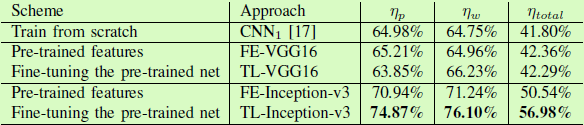
\includegraphics[width=0.8\linewidth]{12}
	\end{center}
	\caption{Comparing the results training form scratch , using deep features via a pre-trained network with no change (FE-VGG16), and classification after fine-tuning a pre-trained network (TL-VGG16, TL-Inception-v3). The best scores are highlighted in bold.(\textit{$\eta_p$} means the patch-to-scan accuracy and \textit{$\eta_n$} means whole-scan accuracy)} 
	\label{fig:long}
	\label{fig:onecol}
\end{figure}

The result shows in figure 6 that pre-trained networks are quite competitive against training from scratch. In this figure, VGG16 and CNN are quite similar, whereas the results for Inception-v3 are similar with the transfer-learned model outperforming the feature extractor. But considering Inception-v3 requires no extra effort and produces similar results with a linear SVM, one may prefer using it to training from scratch and fine-tuning a pre-trained net.

In the next article\cite{araujo2017classification}, the authors designed a specific CNN network which perform image-wise classification in four classes of medical relevance: normal tissue, benign lesion, in situ carcinoma and invasive carcinoma. The proposed CNN architecture is designed to integrate information from multiple histological scales, including nuclei, nuclei organization and overall structure organization. A data augmentation method is adopted to increase the number of cases in this training set. A SVM classification using the features extracted by the CNN is also used for comparison purposes.

The dataset is composed of an extended training set of 249 images, and a separate test set of 20 images. In these datasets, the four classes are balanced. The images were selected so that the pathology classification can be objectively determined from the image contents. An additional
test set of 16 images is provided with images of increased ambiguity, which they denote as extended dataset.

They first normalized the images. First, the colors of the images are converted to optical density (OD) using a logarithmic transformation. Then, they used singular value decomposition (SVD)  to the OD tuples to find the 2D projections with higher variance. The resulting color space transform is then applied to the original image. Finally, the image histogram is stretched so that the dynamic range covers the lower 90\% of the data.

Then they do two kinds of classification: Image-wise classification and CNN patch-wise classification. Image-wise classification first divided the origin image into twelve contiguous non-overlapping patches and then use one of three different patch patch methods: majority voting, maximum probability and sum of probabilities. CNN patch-wise classification used 75\% of the data to do the training and validated on the remaining images.The validation set is randomly selected for each epoch. The training process stops after the stabilization of the validation accuracy with equal weight for all the classes (50 epochs). The authors also used the features extracted by the CNN to train a SVM classifier to do the comparison. The result can be seen in figure 7, 8 and 9.

\begin{figure}[t]
	\begin{center}
		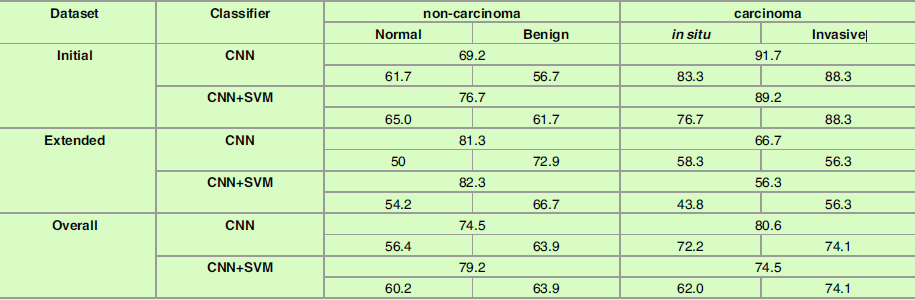
\includegraphics[width=0.8\linewidth]{13}
	\end{center}
	\caption{Patch-wise sensitivity (\%) (2 and 4 classes).} 
	\label{fig:long}
	\label{fig:onecol}
\end{figure}

\begin{figure}[t]
	\begin{center}
		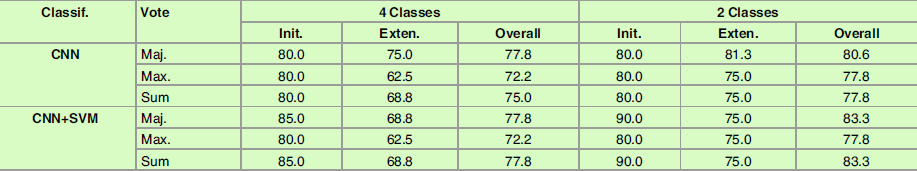
\includegraphics[width=0.8\linewidth]{15}
	\end{center}
	\caption{Image-wise accuracy (\%) using different voting rules (2 and 4 classes).} 
	\label{fig:long}
	\label{fig:onecol}
\end{figure}

\begin{figure}[t]
	\begin{center}
		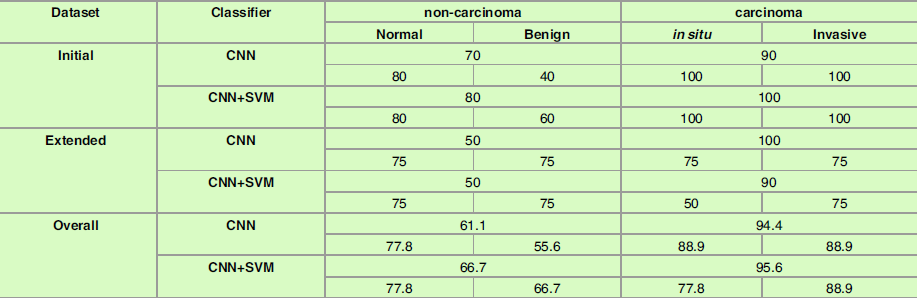
\includegraphics[width=0.8\linewidth]{14}
	\end{center}
	\caption{Image-wise sensitivity (\%) using majority voting (2 and 4 classes).} 
	\label{fig:long}
	\label{fig:onecol}
\end{figure}

In figure 7, we can see the result similar between the CNN and CNN+SVM. But the performance of this network is lower for the extended dataset due to its increased complexity. In figure 8 and 9, we can see that CNN+SVM get the best result with the majority voting method. In comparison, CNN's performance is only better for the extended set using majority voting. In addition, we can see that maximum probability is the worst performing method in both methods, which means that this method is not suit in this case.

\subsection{Some kinds of lung diseases classification}

Lung cancer is notoriously aggressive with a low long-term survival rate. Quantitative analysis in lung nodules using thoracic Computed Tomography(CT) has been a central focus for early cancer diagnosis, where CT phenotype provides a powerful tool to comprehensively capture nodule characteristics. The importance of diagnostically classifying malignant and benign nodules using CT images is to facilitate radiologists for nodule staging assessment and individual therapeutic planning.\cite{shen2015multi}

In the first article\cite{shen2015multi}, the authors used the LIDC-IDRI datasets, which has 1375 nodule pictures(1100 for training and 275 for testing). In order to improve the speed and accuracy, the authors introduced an Multi-scale Convolutional Neural Networks(MCNN) model to do the lung nodule diagnostic classification. This CNN model take multi-scale raw nodule patches and remove the need of any hand-crafted feature engineering work. This network can also deal with noisy data in nodule CT.

Because of the clinical fact that nodule sizes vary remarkably, this network take patches from different scales(3 layers) as inputs in parallel. The parameter is shared between these layers to reduce parameter. When doing the evaluation task, the result is decided by all the layers. The authors use the HOG and uniform LBP descriptor and SVM and RF classifier to do the classification. The result can be seen in figure 6 and figure 7. In figure 7, the \textit{$S_w$} means the size of the cell window for SVM and \textit{$n_{pt}$} means the number of neighbourhood points for LBP.

\begin{figure}[t]
	\begin{center}
		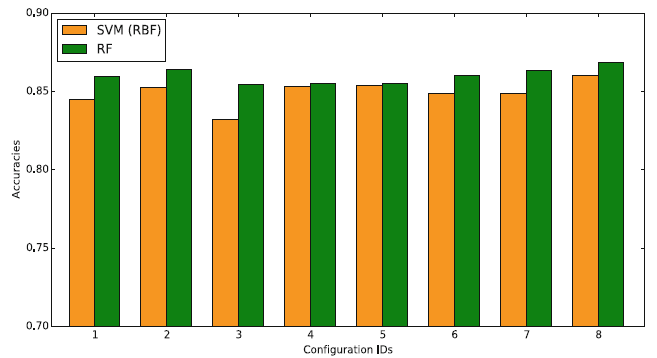
\includegraphics[width=0.8\linewidth]{9}
	\end{center}
	\caption{The classification performance of SVM with the RBF kernel and RF based on features from the MCNN using 8 different configurations. Each configuration is assigned to a unique ID for display convenience} 
	\label{fig:long}
	\label{fig:onecol}
\end{figure}

\begin{figure}[t]
	\begin{center}
		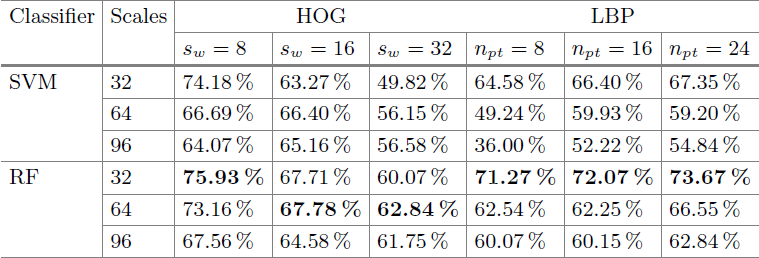
\includegraphics[width=0.8\linewidth]{10}
	\end{center}
	\caption{Performance using the HOG and LBP descriptors with different \textit{$S_w$} and \textit{$n_{pt}$}} 
	\label{fig:long}
	\label{fig:onecol}
\end{figure}

The second article\cite{li2014medical} is about using CNN to classify the ILD patterns. This experiment used an ILD database which contains 113 sets of HRCT images, with 2062 2D regions indicting the ILD category. In order to augment the dataset, the CT slices were divided into half-overlapping image and the only if 75\% percent of its pixels falling inside the regions of interest will be adopted. The dataset thus contains 16220 image patches from 92 HRCT image sets,
including 4348 norm patches, 1047 emphysema patches, 1953 ground glass patches, 2591 fibrosis patches, and 6281 micronodules patches. 

The authors compared their classification results with three other feature extraction approaches: SIFT feature, LBP feature and unsupervised feature learning using RBM. The result can be seen in Figure 8. In this figure, we can see that their customized CNN method achieved the best classification preformance.

\begin{figure}[t]
	\begin{center}
		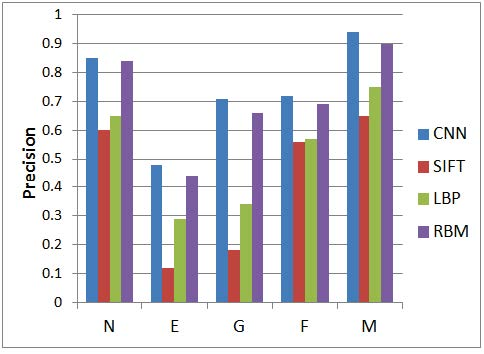
\includegraphics[width=0.8\linewidth]{11}
	\end{center}
	\caption{The classification results comparing proposed customized CNN method with SIFT, LBP and RBM} 
	\label{fig:long}
	\label{fig:onecol}
\end{figure}

\subsection{dental disease classification in X-ray images}

The author found that there is no literature for dental disease classification, so the research group start to use CNN to deal with X-ray images and make some breakthrough. Orthopantomogram (OPG) and Radiovisiography (RVG) x-ray images are the most widely used tools for the diagnoses of dental diseases. Dental caries is one of the most common dental disease worldwide and it has different stages. So the CNN network in this experiment is used to classify mainly 3 classes (dental caries, periapical infection, periodontitis)\cite{prajapaticlassification}.

Because though the radiologists have large dataset of dental x-ray images, these x-ray images have individual privacy issues. So the dataset is very small in this experiment, just have 251 grey images of dimension 1000*1496. So the authors use transfer learning method to do the fine tuning and improve the accuracy very much. They changed some unfrozen layers used for training in order for the pre-trained model to be more adaptive to the training data. 

They first resize these picture to 500*748, and then use 180 of 251 to do the training, 45 images for validation and 26 images for testing purpose. Because of the unavailability of the large dataset, CNN architecture could not perform well in this classification task. After they used transfer learning model to do the fine tuning, the accuracy is increased by 15.39\% compared to pure CNN model, and achieved 88.46\% accuracy, which is very encouraging.

\begin{figure}[t]
	\begin{center}
		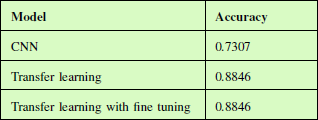
\includegraphics[width=0.8\linewidth]{2}
	\end{center}
	\caption{The comparison of different models} 
	\label{fig:long}
	\label{fig:onecol}
\end{figure}

\begin{figure}[t]
	\begin{center}
		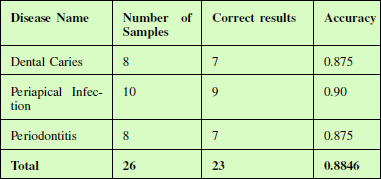
\includegraphics[width=0.8\linewidth]{3}
	\end{center}
	\caption{Experimental results for transfer learning model} 
	\label{fig:long}
	\label{fig:onecol}
\end{figure}

\subsection{intima-media boundary segmentation}

Automated classification of human anatomy is an important prerequisite for many computer-aided diagnosis systems. The spatial complexity and variability of anatomy throughout the human body makes classification difficult. So the authors want to use CNN to do this classification. In this paper, the authors choose to use 4298 separate axial 2D key images to learn 5 anatomical classes(neck, lungs, liver, pelvis and legs)\cite{roth2015anatomy}.

When applying the CNN to build the anatomy-specific classifier for CT images, because the authors want to classify these picture to 5 classes, so they choose 5 cascaded layers. All the convolutional filter kernel elements are trained from the data in a supervised fashion. In order to avoid overfitting, the fully-connected layers are constrained, using the \textit{DropOut} method. The datasets are from the Picture Archiving and Communication System (PACS) of the Clinical Center of the National Institutes of Health. In order to enrich their data, they use spatial deformations to each image, using random translation, rotations and non-rigid deformations, which lead their datasets from hundred's picture to near 100 thousand pictures. Before import into the CNN, the author resize all the picture to 256*256 pixels.The authors use 80\% of their total dataset to train the CNN and reserve 20\% to do the test. After doing the experiments, the accuracy of this net can reach 94.1\%, which can be seen in figure 4.This classification
result is achieved in less than 1 minute on a modern desktop computer and GPU card (Dell Precision T7500,
24GB RAM, NVIDIA Titan Z).

\begin{figure}[t]
	\begin{center}
		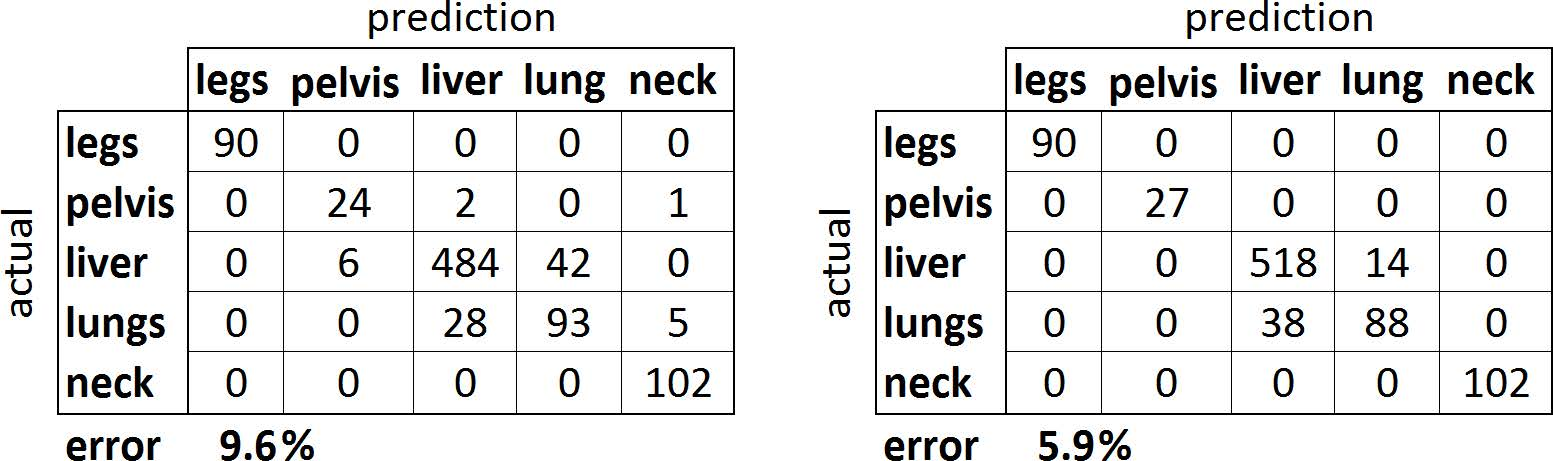
\includegraphics[width=0.8\linewidth]{1}
	\end{center}
	\caption{Confusion matrices on the original test images before and after data augmentation.} \label{fig:long}
	\label{fig:onecol}
\end{figure}

\subsection{Conclusion}

In this part, I aimed to address to know how the CNN can be used on the medical image classification and the result these experiments made. My experiment, based on 4 distinct medical imaging applications from different imaging modality systems, have demonstrated that deep CNN are useful for medical image analysis. If the training data is limited, the fine-tuned CNN can perform better than fully trained CNN. I think the potential of CNNs for medical imaging applications is confirmed because both deeply fine-tuned CNNs and fully trained CNNs can outperform the corresponding handcrafted alternatives. We can also see that the speed is depend on the devices, the more powerful the graphics is, the quicker the CNN network use to train.

%------------------------------------------------------------------------


{\small
\bibliographystyle{ieee}
\bibliography{egbib}
}

\end{document}
